\section{The DOI Data Model}
\label{sec:DataModel}
In a typical AOI-based analysis, analysts divide a visual stimulus into sub-regions critical in testing a hypothesis. By analogy, DOIs are subsets of a visualization's underlying data. For example, in a network visualization, DOIs may be individual nodes or clusters of nodes. In a 3D scene-rendering they may be individual objects or components of objects that are part of the scene. When DOIs have corresponding visual representations in the visualization's output, then gaze coordinates can be mapped to DOIs via these representations. 

We can approximate a general visualization's data model using the generic entity-attribute-value (EAV) data model~\cite{deran1991entity}: different types of data entities are described by combinations of attribute-value pairs. More complex data models can be captured by extending the EAV paradigm with classes and relationships (EAV/CR), meaning that attribute values can themselves be entities. 

As such, a visualization's underlying data model will define entity and attribute types, attribute value ranges, and classes and relationships between entities, while a visualization that encodes it will define how these are translated into visual output. A specific instance of such a data model (i.e., a data set) will contain a configuration of entities, attributes, values, and relationships that conform to the data model. 

DOIs are created onto data instances as subsets of data, and are characterized by that data subset's specific attributes and values (Fig.~\ref{fig:dataModel}, `DOI data subsets'). For example, DOIs could be defined in a node-link visualization of interacting proteins for each node and may be described by attributes such as label, type, degree of activation, or sequence. However, DOIs could also be created for larger subsets of data, such as for example a meta-node or pathway if the node-link visualization had a hierarchical structure. In this case, the DOI would encompass data from multiple entities. Deciding how to split a visualization's underlying data into DOIs (e.g., individual objects or groups of objects) is up to the instrumenter and depends on two factors: what the data models is, and which data subsets make sense as visual units in the instrumented visualization. 

In practice, DOIs are defined by instrumenting a visualization's code~\cite{alam15analyzing}. First, upon loading a dataset, DOIs can be created for particular subsets of it. Second, rendering calls need to be mirrored such that whenever data corresponding to a DOI is shown on the screen, its visual representation (i.e., shape, position) is monitored. Then, gazes obtained from an eye-tracker are matched to these visual representations and in turn to their associated DOIs. 

By instrumenting visualization code we specify how a visualization's underlying data model should be assigned to DOIs. However, DOIs are created at run-time from specific data sets rather than from abstract data models. For example, when instrumenting a network visualization, we would define that each node in the network should be a DOI, but ultimately, specific DOIs get created at run-time from a specific dataset and specific visualization instance. This process is shown in Figure~\ref{fig:dataModel}.

Both Bernhard et al.~\cite{bernhard2014gaze} and Alam et al.~\cite{alam15analyzing} compute candidate objects a user is likely to have viewed when fixating on a particular coordinate, by considering which objects intersect a small area around the user's fixation, rather than just the fixation itself. Ultimately, Bernhard et al. report only the object closest to the fixation, while Alam et al. report all viewing candidates.  Both authors argument their decision. For a more general description of a DOI data model we will consider Alam et al.'s approach. 

As such, the DOI instrumentation will report which DOIs a user has viewed over time with each of their fixations (Figure~\ref{fig:dataModel}). Each fixation will have a duration, and may be associated with one viewed DOI, multiple viewed DOIs, or no viewed DOI. Moreover, our confidence that a DOI was indeed the locus of the user's attention will be inversely proportional to the distance from that DOI to the fixation, and thus variable. For example, in Figure 5, we are less confident that the user viewed DOI2 during their fifth fixation, than we are that they viewed DOI1 during their first.  

\begin{figure}[!htb]
  \centering
  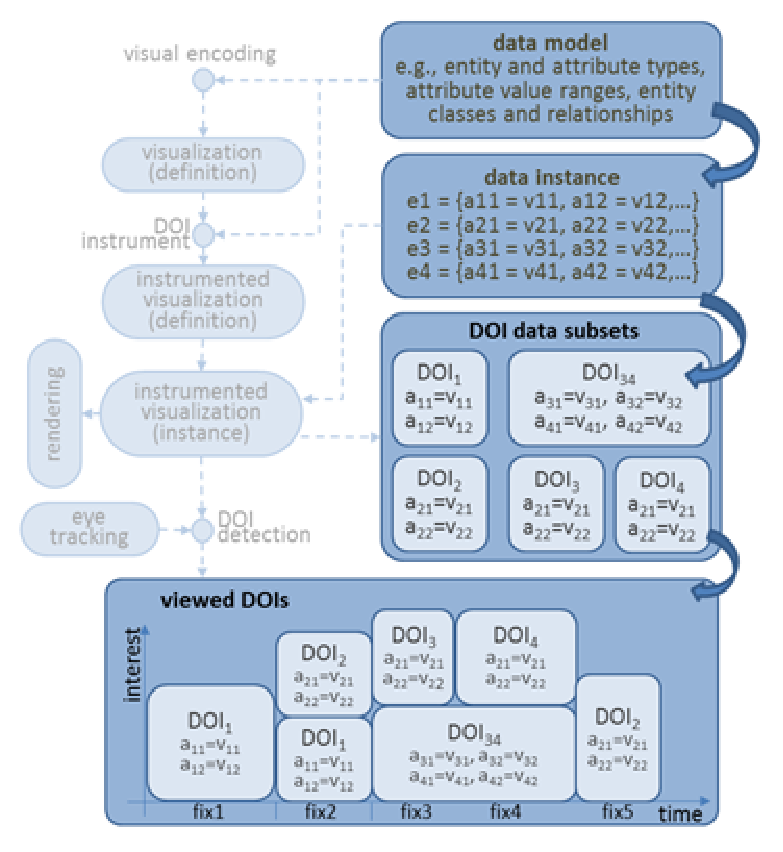
\includegraphics[width=\linewidth]{images/DOIDataModel.eps}
  \caption{DOI data model, DOI definition and collection. }
	\label{fig:dataModel}
\end{figure}



\subsection{AOI vs DOI}
\label{sec:AOIvDOI}
There are signficant differences between AOIs and DOIs. Describing them helps emphasize the properties of DOI data and motivates the need for new research in DOI analysis.

\textbf{\underline{Definition:}}Analysts can define AOIs over stimuli either before the experiment or during the analysis phase. The AOIs are defined in stimulus or image space. (e.g.: an image region with particular semantic meaning or that is relevant for a task). Conversely, DOIs are defined over the data model by instrumenting the code that translates data into visualization.   (e.g., in a graph visualization DOIs could be defined for each node, for edges, or for groups of nodes (i.e., nodes that satisfy a certain condition over their attributes).

\textbf{\underline{Data scale and granularity:}}AOIs tend to be large and sparse, and AOI analysis work with a small number of AOIs. Conversely, DOIs are many, small, and because collection doesn't rely on manual coding, can be collected over long periods of time. Thus, a DOI analysis can involve thousands of DOIs that a user looked at during a one hour analysis.

\textbf{\uline{DOIs have explicit properties derived from the underlying data:}} AOIs have implicit properties known to the analyst but generally not expressed explicitly. For example, in a node-link visualization of movie data, a cluster of nodes can an AOI where that cluster may represent a group movie which are only of action genre. Instead, DOIs properties are explicit and are automatically derived the underlying/instrumented data. For the same example given above, each node may represent a movie and each movie may have been categorized under multiple genres. 

\textbf{\underline{Time requirement of analysis sessions:}} AOI analysis generally requires longer sessions of analysis. DOI analysis is relatively much shorter than AOI-based analysis.

\textbf{\underline{Requirement of instrumentations:}} AOI analyses generally do to require instrumentations into the source code. Moreover, instrumentation over source is prerequisite for DOI analyses. 

\textbf{\underline{DOI data is probabilistic:}}  Gazes on AOIs are generally concrete. We can certainly report which AOIs received how many gaze points. On the contrary, gazes on DOIs are generally in fractions. Different algorithms or scoring methods yield different fractional scores to DOIs. Eye-trackers are generally imprecise and produces low-resolution data. Considering the node-link visualization example, if a gaze point lands in between two or more graph-nodes then, segregation among graph-nodes to relate with that gaze point becomes a challenge. 

DOIs can be defined hierarchically or in groups: Each node in a graph can have its own DOI, but groups of nodes can have their own DOI as well, etc.

\subsection{DOI Exemplification}
We give examples DOIs in four research domains: movie-data, education, construction-data and proteomics-data. Examples are illustrated in Table~\ref{tab:ExampleDOI}. 

For movie-data, suppose we want to define a DOI for a movie. So we take domain $M$ for movies and $R$ for ratings. We get a data element $d \in M \times R$. Now we inject attributes such as movie title ($a_1$), release date ($a_2$), and rating ($a_3$). We set the condition $C= \text{rating} \geq 5.0$. So we have a movie DOI set $\text{DOI}_{movie} = \prod_{a_1,a_2,a_3}\sigma_{\text{rating} \geq 5.0} M \times R$. Thus, an element $d_i \in \text{DOI}_{movie}$ would be a tuple : $d_i =< a_1, a_2, a_3>$. 

We demonstrate DOI definition for education domain. We consider a scenario where a student is learning from many learning materials such as books, articles, lectures in possible two formats: visual and auditory. For simplicity we avoid auditory formats. Visual learning elements can be static or dynamic. Static elements include textual descriptions and images. Dynamic elements are videos or animated versions of static diagrams. For instance, a scientific paper can have domains such as abstract ($T_{Abs}$), introduction ($T_{Intro}$, conclusions ($T_{Concl}$), images ($I$), tables ($Tab$), equations ($Eq$). An example DOI can be title of image which is referenced in the introduction. In this case, the condition is $C=$referenced and the attributes might be title and word count. So we get $\text{DOI} = \prod_{(title, wordcount)} \sigma_{(\text{referenced})} I \times T_{Intro}$. 

Construction-data consists of shop drawings, material-data, samples and product-data used by architectures and engineers to verify feasibility of any architectural project. A shop drawing may contain a design of a building from multiple perspectives. For a particular perspective, there might be labels indicating part to the buildings and what materials are used. For example, we denote such shop drawing as $S$ and perspectives as $P$. Now we define a DOI which contains attributes $A$ with compartment names $a_1$ and materials names $a_2$. Then we inject the condition $C=$ top view of the design. So we get a $DOI_{construction} = \prod_{a_1,a_2} \sigma_{topview} S \times P$ which will produce compartment of the design DOIs with compartment names and materials used. 

\begin{table*}[htbp]
	\centering
		\begin{tabular}{|c|c|c|l|l|}
			\hline
	Example Model & Domains & Attributes & Condition& DOI-tuple\\\hline
	Movie-Data & \shortstack{Movies,\\ Actors} & \shortstack{Movie title,\\ release date,\\ ratings}& $rating \geq 5.0$& $<\text{Star Wars}, 1977, 8.7>$ \\\hline
	Education & \shortstack{Article sections,\\ images} & \shortstack{Section title,\\ word count} & $image_i \in paragraph_p$& $<\text{Introduction}, 379>$ \\\hline
	Construction-Data & \shortstack{Shop drawings,\\ perspectives} & \shortstack{Drawing section name,\\ materials used} & $perspective_i =topview$& $<\text{Bat-cave}, \text{limestone}>$ \\\hline
	Proteomics & X& X& X& X \\\hline
		\end{tabular}
		\caption{Examples of DOIs. i)}
		\label{tab:ExampleDOI}
\end{table*} 







